% Recuerda incluir en el preámbulo:
% \usetikzlibrary{arrows.meta, babel}

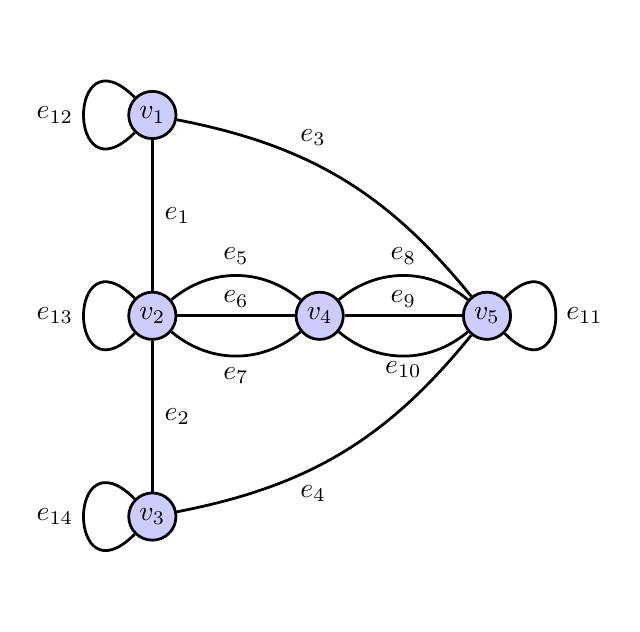
\begin{tikzpicture}[
  scale=0.85, 
  auto=left,
  every node/.style={circle, fill=blue!20, draw=black, line width=1pt, inner sep=2pt, minimum size=6mm}
]

  % Posicionamiento horizontal de vértices
  \node (v1) at (0,3) {$v_1$};
  \node (v3) at (0,-3) {$v_3$};
  \node (v2) at (0,0) {$v_2$};
  \node (v4) at (2.5,0) {$v_4$};
  \node (v5) at (5,0) {$v_5$};

  % Bucles en v1, v2 y v3
  \path[line width=1pt] (v1) edge[loop left, out=135, in=225, looseness=7] node[draw=none, fill=none, left, inner sep=2pt] {$e_{12}$} (v1);
  \path[line width=1pt] (v2) edge[loop left, out=135, in=225, looseness=7] node[draw=none, fill=none, left, inner sep=2pt] {$e_{13}$} (v2);
  \path[line width=1pt] (v3) edge[loop left, out=135, in=225, looseness=7] node[draw=none, fill=none, left, inner sep=2pt] {$e_{14}$} (v3);

  % Aristas verticales iniciales
  \draw[line width=1pt] (v1) -- node[draw=none, fill=none, right, inner sep=1pt] {$e_1$} (v2);
  \draw[line width=1pt] (v2) -- node[draw=none, fill=none, right, inner sep=1pt] {$e_2$} (v3);

  % Conexiones curvas v1 -> v5 y v3 -> v5
  \draw[line width=1pt] (v1) to[bend left=20] node[draw=none, fill=none, above, inner sep=1pt, pos=0.4] {$e_3$} (v5);
  \draw[line width=1pt] (v3) to[bend right=20] node[draw=none, fill=none, below, inner sep=1pt, pos=0.4] {$e_4$} (v5);

  % Múltiples aristas entre v2 y v4
  \draw[line width=1pt] (v2) to[bend left=40] node[draw=none, fill=none, above, yshift=-2pt] {$e_5$} (v4);
  \draw[line width=1pt] (v2) -- node[draw=none, fill=none, above, yshift=-3pt] {$e_6$} (v4);
  \draw[line width=1pt] (v2) to[bend right=40] node[draw=none, fill=none, below, yshift=2pt] {$e_7$} (v4);

  % Múltiples aristas entre v4 y v5
  \draw[line width=1pt] (v4) to[bend left=40] node[draw=none, fill=none, above, yshift=-2pt] {$e_8$} (v5);
  \draw[line width=1pt] (v4) -- node[draw=none, fill=none, above, yshift=-3pt] {$e_9$} (v5);
  \draw[line width=1pt] (v4) to[bend right=40] node[draw=none, fill=none, below, yshift=5.5pt] {$e_{10}$} (v5);

  % Bucle en v5
  \path[line width=1pt] (v5) edge[loop right, out=45, in=-45, looseness=7] node[draw=none, fill=none, right, pos=0.5, inner sep=2pt] {$e_{11}$} (v5);

\end{tikzpicture}
